%-----------------------------------------------------------------------
% Beginning of chapter.tex
%-----------------------------------------------------------------------
%
%  This is a sample file for use with AMS-LaTeX.  It provides an example
%  of how to set up a file for a book to be typeset with AMS-LaTeX.
%
%  This is the driver file.  Separate chapters should be included at
%  the end of this file.
%
%  ***** DO NOT USE THIS FILE AS A STARTER FOR YOUR BOOK. *****
%  Follow the guidelines in the file chapter.template.
%
%%%%%%%%%%%%%%%%%%%%%%%%%%%%%%%%%%%%%%%%%%%%%%%%%%%%%%%%%%%%%%%%%%%%%%%%

\documentclass[11pt,a4paper]{memoir}
\chapterstyle{demo}
\epigraphfontsize{\small\itshape}
\setlength\epigraphwidth{8cm}
\setlength\epigraphrule{0pt}
\epigraphfontsize{\small\itshape}
%\includeonly{preface,chap1,biblio}

%\numberwithin{section}{chapter}
%\numberwithin{equation}{chapter}

% Include macros here
%=================================================
% Packages
%=================================================

%\usepackage{fixltx2e}
\usepackage[usenames,dvipsnames]{xcolor}
%\usepackage{fancyhdr}
\usepackage{amsmath,amsfonts,amsbsy,amsgen,amscd,mathrsfs,amssymb,amscd}
\usepackage{amsthm}
\usepackage{bm}
\usepackage{url}
\usepackage[UKenglish]{babel}
\usepackage{eurosym}
\usepackage{tikz}
\usepackage{caption}
\usetikzlibrary{matrix,arrows,shapes,calc,3d}
\usepackage{tikz-3dplot}
\tdplotsetmaincoords{60}{110}
\pgfmathsetmacro{\rvec}{.8}
\pgfmathsetmacro{\thetavec}{30}
\pgfmathsetmacro{\phivec}{60}

\tikzset{mynode/.style = {
    % The shape
    circle,
    % The size
    minimum size=2pt,
    % The color
    draw=black, fill=black}
}
\tikzset{vertex/.style={shape=circle, % style for a vertex
                        minimum size=3pt,
                        fill=gray,
                        inner sep = 0pt}}  

% \usepackage{3dplot}
% \tdplotsetmaincoords{60}{110}
%\usepackage{subfig}
\usepackage{microtype}
\usepackage{enumitem}
\usepackage{listings}
\definecolor{darkblue}{rgb}{0,0,.75}

\usepackage[many]{tcolorbox}
\tcbuselibrary{listings}

\definecolor{light-gray}{rgb}{0.96,0.96,0.96}
\definecolor{kwgreen}{rgb}{0,0.5,0}
\definecolor{cogreen}{rgb}{0.25,0.5,0.5}
\definecolor{mygreen}{rgb}{0,0.5,0.125}
\definecolor{equalsign}{rgb}{0.66,0.13,1}
\definecolor{darkred}{rgb}{0.75,0.16,0.37}

\lstloadlanguages{Python} %use listings with Python
%\lstset{literate={==}{{\color{equalsign}==}} {\*}{{\color{equalsign}\*}}}
%\lstnewenvironment{PseudoCode}[1][]
% the space reserved between for the ``In'' numbers and the code
\newlength\inwd
\setlength\inwd{1.7cm}

\newcounter{ipythcntr}

\newtcblisting{ipythonnb}[1][\theipythcntr]{
  enlarge left by=\inwd,
  width=\linewidth-\inwd,
  enhanced,
  boxrule=0.4pt,
  boxsep=0pt,
  left=2pt,
  top=0pt,
  colback=light-gray,
  listing only,
  top=0pt,
  bottom=0pt,
  arc=1pt,
  overlay={
    \node[
      anchor=north east,
      text width=\inwd,
      font=\footnotesize\ttfamily\color{blue!50!black},
      inner ysep=2.5mm,
      inner xsep=0pt,
      outer sep=0pt
      ] 
      at (frame.north west)
      {\stepcounter{ipythcntr}In [#1]:};
  }
  listing style=Python,
  listing options={
    basicstyle=\scriptsize\ttfamily\color{black},
    language=Python,
    escapechar=£,
    showstringspaces=false,
    commentstyle=\color{cogreen},
    keywordstyle=\bfseries\color{kwgreen},
    stringstyle=\color{darkred},
    numberstyle=\color{kwgreen},
    identifierstyle=\color{black},
    %emph={from,import,as},          % Custom highlighting
    otherkeywords={0,1,2,3,4,5,6,7,8,9,\*,==,<=,>=,+,-,\%},
    emph={*,==,<=,>=,+,-,\%},    
    emphstyle=\color{equalsign},
    extendedchars=true,
  },
}

\newtcblisting{ipythonnbout}[1][\theipythcntr]{
  enlarge left by=\inwd,
  width=\linewidth-\inwd,
  enhanced,
  boxrule=0pt,
  boxsep=0pt,
  left=2pt,
  top=0pt,
  colback=white,
  listing only,
  top=0pt,
  bottom=0pt,
  frame hidden,
  overlay={
    \node[
      anchor=north east,
      text width=\inwd,
      font=\footnotesize\ttfamily\color{red},
      inner ysep=2.5mm,
      inner xsep=0pt,
      outer sep=0pt
      ] 
      at (frame.north west)
      {\stepcounter{ipythcntr}Out [#1]:};
  }
  listing style=Python,
  listing options={
    basicstyle=\scriptsize\ttfamily\color{black},
    language=Python,
    escapechar=£,
    showstringspaces=false,
    commentstyle=\color{cogreen},
    keywordstyle=\bfseries\color{kwgreen},
    stringstyle=\color{darkred},
    numberstyle=\color{kwgreen},
    identifierstyle=\color{black},
    %emph={from,import,as},          % Custom highlighting
%    otherkeywords={as,0,1,2,3,4,5,6,7,8,9,\*,==,<=,>=,+,-},
%    emph={*,==,<=,>=,+,-},    
%    emphstyle=\color{equalsign},
    extendedchars=true,
    %literate={#}{{\#}},
  },
}

\newtcblisting{ipythonnboutno}{
  enlarge left by=\inwd,
  width=\linewidth-\inwd,
  enhanced,
  boxrule=0pt,
  boxsep=0pt,
  left=2pt,
  top=0pt,
  colback=white,
  listing only,
  top=0pt,
  bottom=0pt,
  frame hidden,
  overlay={
    \node[
      anchor=north east,
      text width=\inwd,
      font=\footnotesize\ttfamily\color{red},
      inner ysep=2.5mm,
      inner xsep=0pt,
      outer sep=0pt
      ] 
      at (frame.north west)
      {};
  }
  listing style=Python,
  listing options={
    basicstyle=\scriptsize\ttfamily\color{black},
    language=Python,
    escapechar=£,
    showstringspaces=false,
    commentstyle=\color{cogreen},
    %keywordstyle=\bfseries\color{kwgreen},
    stringstyle=\color{darkred},
    numberstyle=\color{kwgreen},
    identifierstyle=\color{black},
    %emph={from,import,as},          % Custom highlighting
    %otherkeywords={as,0,1,2,3,4,5,6,7,8,9,\[,\]},
    %emph={[,]},    
    %emphstyle=\color{black},
    extendedchars=true,
    %literate={#}{{\#}},
  },
}


%{\lstset{language=Matlab,basicstyle=\small, keywordstyle=\color{darkblue},numbers=none,xleftmargin=.04\textwidth,mathescape,frame=single,#1}}
%{}
%\usepackage[]{algorithm2e}
%\usepackage{mcode}
\usepackage{multicol}

%\usepackage[draft]{changes}
%\definechangesauthor[color=blue]{ml}
%\definechangesauthor[color=red]{da}
% \usepackage{trackchanges}
% \addeditor{ml}
% \addeditor{da}

\definecolor{dark-gray}{gray}{0.3}
\definecolor{dkgray}{rgb}{.4,.4,.4}
\definecolor{dkblue}{rgb}{0,0,.5}
\definecolor{medblue}{rgb}{0,0,.75}
\definecolor{rust}{rgb}{0.5,0.1,0.1}

\usepackage[colorlinks=true]{hyperref}
\hypersetup{urlcolor=Blue}
\hypersetup{citecolor=Black}
\hypersetup{linkcolor=dark-gray}

%\usepackage{setspace}
\usepackage{graphicx}
%\usepackage{multicol}
\usepackage{booktabs,longtable,tabu} % Nice tables
\setlength{\tabulinesep}{1pt}
\usepackage{multirow} % More control over tables
\usepackage{float}
\usepackage[T1]{fontenc}
%\usepackage{quotchap}

% Fonts
\usepackage{times}
%\usepackage{fourier}
%\usepackage[no-math]{fontspec}
%\setmainfont{optima}
%\usepackage{charter}
\usepackage{bm} % boldmath must be called after the package

%=================================================
% Paths
%=================================================

\graphicspath{{figures/}}

%=================================================
% Formatting
%=================================================

%\sloppy % Helps with margin justification

%%% Further font changes
\newcommand{\lang}{\textit}
\newcommand{\titl}{\textsl}
\newcommand{\term}{\emph}

%%% Equation numbering
\numberwithin{equation}{section} 

%%% Typesetting
\providecommand{\mathbold}[1]{\bm{#1}}  % Must be after 'fourier'
                                % package loads
%%% Annotations
\newcommand{\notate}[1]{\textcolor{red}{\textbf{[#1]}}}

%=================================================
% Theorem environment
%=================================================

\newtheorem{bigthm}{Theorem}
\renewcommand{\thebigthm}{\Roman{bigthm}}

\newtheorem{theorem}{Theorem}[section]
\newtheorem{lemma}[theorem]{Lemma}
\newtheorem{sublemma}[theorem]{Sublemma}
\newtheorem{proposition}[theorem]{Proposition}
\newtheorem{fact}[theorem]{Fact}
\newtheorem{result}[theorem]{Result}
\newtheorem{conjecture}[theorem]{Conjecture}
\newtheorem{corollary}[theorem]{Corollary}

\newtheorem{problem}[theorem]{Problem}
\newtheorem{solution}[theorem]{Solution}

\theoremstyle{definition}

\newtheorem{definition}[theorem]{Definition}
\newtheorem{example}[theorem]{Example}
\newtheorem{remark}[theorem]{Remark}

\newenvironment{mainthm}{\par\textsc{Main theorem.}\it}{\par}
\renewcommand{\thebigthm}{\Alph{bigthm}}

%=================================================
% Symbols
%=================================================

%%% Old symbols with new names
\newcommand{\oldphi}{\phi}
\renewcommand{\phi}{\varphi}

\newcommand{\eps}{\varepsilon}
\newcommand{\e}{\varepsilon}

%\newcommand{\oldmid}{\mid}
\renewcommand{\mid}{\mathrel{\mathop{:}}} 

%%% New symbols
\newcommand{\defby}{\overset{\mathrm{\scriptscriptstyle{def}}}{=}}
\newcommand{\half}{\tfrac{1}{2}}
\newcommand{\third}{\tfrac{1}{3}}

\newcommand{\sumnl}{\sum\nolimits}

\newcommand{\defeq}{\ensuremath{\mathrel{\mathop{:}}=}} % Definition-equals
\newcommand{\eqdef}{\ensuremath{=\mathrel{\mathop{:}}}} % Equals-definition

%%% Constants
\newcommand{\cnst}[1]{\mathrm{#1}} 
\newcommand{\econst}{\mathrm{e}}
\newcommand{\iunit}{\mathrm{i}}

\newcommand{\onevct}{\mathbf{e}} % All ones vector
\newcommand{\zerovct}{\vct{0}} % Zero vector

\newcommand{\Id}{\mathbf{I}}
\newcommand{\onemtx}{\bm{1}}
\newcommand{\zeromtx}{\bm{0}}

%%% Sets
\newcommand{\coll}[1]{\mathscr{#1}}
\newcommand{\sphere}[1]{S^{#1}}
\newcommand{\ball}[1]{B^{#1}}
\newcommand{\Grass}[2]{\mathbb{G}(#1,#2)}
\providecommand{\mathbbm}{\mathbb} % In case we don't load bbm
\newcommand{\Rplus}{\mathbbm{R}_{+}}
\newcommand{\R}{\mathbbm{R}}
\newcommand{\C}{\mathbbm{C}}
\newcommand{\N}{\mathbbm{N}}
\newcommand{\FF}{\mathbbm{F}}
\newcommand{\struct}{\mathcal{S}}

% Group theory
\newcommand{\stab}{\mathrm{stab}}

% Algebra
\newcommand{\End}{\mathrm{End}}
\newcommand{\Hom}{\mathrm{Hom}}
\newcommand{\Mult}{\mathrm{Mult}}

% Set operations
\newcommand{\polar}{\circ}
\newcommand{\closure}{\overline}
\newcommand{\prtensor}{\,\hat{\otimes}\,}

%%% Real and complex analysis
\newcommand{\abs}[1]{\left\vert {#1} \right\vert}
\newcommand{\abssq}[1]{{\abs{#1}}^2}

\newcommand{\sgn}[1]{\operatorname{sgn}{#1}}
\newcommand{\real}{\operatorname{Re}}
\newcommand{\imag}{\operatorname{Im}}
\newcommand{\pos}{\operatorname{Pos}}
\newcommand{\shrink}{\operatorname{Shrink}}

\newcommand{\diff}[1]{\mathrm{d}{#1}}
\newcommand{\idiff}[1]{\, \diff{#1}}

\newcommand{\gradd}{\mathrm{grad }} % Conflicts w/SIAM styles?
\newcommand{\divv}{\mathrm{div }}
\newcommand{\subdiff}{\partial}

%%% Optimization

\newcommand{\minimize}{\text{minimize}\quad}
\newcommand{\maximize}{\text{maximize}\quad}
\newcommand{\subjto}{\quad\text{subject to}\quad}
\newcommand{\find}{\text{find}\quad}
\newcommand{\suchthat}{\quad\text{such that}\quad}

\newcommand{\argmin}{\operatorname*{arg\; min}}
\newcommand{\argmax}{\operatorname*{arg\; max}}
\newcommand{\dom}{\mathrm{dom} }

%%% Probability & measure

\newcommand{\Prob}{\mathbbm{P}}
\newcommand{\Probe}[1]{\Prob\left({#1}\right)}
\newcommand{\Expect}{\operatorname{\mathbb{E}}}

\newcommand{\St}{\operatorname{St}}

%\newcommand{\normal}{\textsc{Normal}}
\newcommand{\normal}{N}
\newcommand{\uniform}{\textsc{Uniform}}
\newcommand{\erf}{\operatorname{erf}}

\DeclareMathOperator{\rvol}{rvol}
\DeclareMathOperator{\Var}{Var}
\DeclareMathOperator{\Gl}{Gl}
\newcommand{\diag}{\operatorname{diag}}

%%% Vector and matrix operators
\newcommand{\vct}[1]{\mathbold{#1}}
\newcommand{\mtx}[1]{\mathbold{#1}}
\newcommand{\Eye}{\mathbf{I}}

\newcommand{\transp}[1]{#1^{T}}
\newcommand{\trans}{\top}
\newcommand{\adj}{*}
\newcommand{\psinv}{\dagger}

\newcommand{\lspan}[1]{\operatorname{span}{#1}}

\newcommand{\range}{\operatorname{range}}
\newcommand{\colspan}{\operatorname{colspan}}

%\newcommand{\rank}{\operatorname{rank}}
\newcommand{\nullity}{\operatorname{null}}
%\newcommand{\ker}{\operatorname{ker}}
\newcommand{\im}{\operatorname{im}}
%\newcommand{\span}{\operatorname{span}}

%\newcommand{\diag}{\operatorname{diag}}
\newcommand{\trace}{\operatorname{tr}}

\newcommand{\supp}[1]{\operatorname{supp}(#1)}
\newcommand{\sign}[1]{\operatorname{sign}(#1)}

\newcommand{\smax}{\sigma_{\max}}
\newcommand{\smin}{\sigma_{\min}}

\newcommand{\nnz}{\operatorname{nnz}}
\renewcommand{\vec}{\operatorname{vec}}

\newcommand{\Proj}{\ensuremath{\mtx{\Pi}}} % Projection operator

%%% Semidefinite orders
\newcommand{\psdle}{\preccurlyeq}
\newcommand{\psdge}{\succcurlyeq}

\newcommand{\psdlt}{\prec}
\newcommand{\psdgt}{\succ}

%%% Mensuration: inner products and norms

% TeX does not like either \newcommand or \renewcommand for these
% two macros.  There is probably a good reason not to use them via
% \def, but I don't know it.  
%\newcommand{\<}{\langle} 
%\newcommand{\>}{\rangle}
\newcommand{\ip}[2]{\langle {#1}, {#2} \rangle}
% --deleted the \left and \right-- Dennis
% \newcommand{\ip}[2]{\left\langle {#1},\ {#2} \right\rangle}
\newcommand{\absip}[2]{\abs{\ip{#1}{#2}}}
\newcommand{\abssqip}[2]{\abssq{\ip{#1}{#2}}}
\newcommand{\tworealip}[2]{2 \, \real{\ip{#1}{#2}}}

%\newcommand{\norm}[1]{\left\Vert {#1} \right\Vert}
\newcommand{\norm}[1]{\Vert {#1}\Vert}
\newcommand{\normsq}[1]{\norm{#1}^2}

\newcommand{\lone}[1]{\norm{#1}_{\ell_1}}
\newcommand{\smlone}[1]{\|#1\|_{\ell_1}}
\newcommand{\linf}[1]{\norm{#1}_{\ell_\infty}}
\newcommand{\sone}[1]{\norm{#1}_{S_1}}
\newcommand{\snorm}[1]{\sone{#1}}
\newcommand{\wnnorm}[1]{\norm{#1}_{*,\vct{w}}}
\newcommand{\wnnormd}[1]{\norm{#1}^*_{\vct{w}}}
\DeclareMathOperator{\dist}{dist}

% Fixed-size inner products and norms are useful sometimes
\newcommand{\smip}[2]{\bigl\langle {#1}, \ {#2} \bigr\rangle}
\newcommand{\smabsip}[2]{\bigl\vert \smip{#1}{#2} \bigr\vert}
\newcommand{\smnorm}[2]{{\bigl\Vert {#2} \bigr\Vert}_{#1}}

% Specific norms that are used frequently
\newcommand{\enormdangle}{{\ell_2}}
\newcommand{\enorm}[1]{\norm{#1}}
\newcommand{\enormsm}[1]{\enorm{\smash{#1}}}

\newcommand{\enormsq}[1]{\enorm{#1}^2}

\newcommand{\fnorm}[1]{\norm{#1}_{\mathrm{F}}}
\newcommand{\fnormsq}[1]{\fnorm{#1}^2}

\newcommand{\pnorm}[2]{\norm{#2}_{#1}}
%\newcommand{\snorm}[1]{\norm{#1}_*}

\newcommand{\triplenorm}[1]{\left\vert\!\left\vert\!\left\vert {#1} \right\vert\!\right\vert\!\right\vert} 

\newcommand{\flag}[2]{{#1 \brack #2}}

% Special cones
\newcommand{\Feas}{\mathcal{F}}
\newcommand{\Desc}{\mathcal{D}}

\newcommand{\sdim}{\delta}
\newcommand{\sdimw}{\delta^*}
% \newcommand{\sdimw}{\tilde{\delta}}
\newcommand{\ddt}[1]{\dot{#1}}
\DeclareMathOperator{\Circ}{Circ}

%%% Differential geometry
\newcommand{\Cinf}{C^{\infty}}
\newcommand{\Tensf}{\mathcal{T}}
\newcommand{\Vbundle}{\mathcal{X}}
\newcommand{\Christ}[3]{\Gamma_{{#1}{#2}}^{#3}}

% Stuff to be sorted in somewhere
\DeclareMathOperator{\Lip}{Lip}

\newcommand{\IR}{\mathbbm{R}}
\newcommand{\veps}{\varepsilon}
\newcommand{\mA}{\mathcal{A}}
\newcommand{\mB}{\mathcal{B}}
\newcommand{\mC}{\mathcal{C}}
\newcommand{\mD}{\mathcal{D}}
\newcommand{\mE}{\mathcal{E}}
\newcommand{\mI}{\mathcal{I}}
\newcommand{\mM}{\mathcal{M}}
\newcommand{\mN}{\mathcal{N}}
\newcommand{\mL}{\mathcal{L}}
\newcommand{\mV}{\mathcal{V}}
\newcommand{\bface}{\overline{\mathcal{F}}}
\newcommand{\face}{\mathcal{F}}
\newcommand{\relint}{\operatorname{relint}}
\newcommand{\relcl}{\operatorname{relcl}}
\newcommand{\cone}{\operatorname{cone}}
\newcommand{\lin}{\operatorname{lin}}
\newcommand{\Gr}{\operatorname{Gr}}
\newcommand{\powerset}{\mathscr{P}}
\newcommand{\hd}{{\operatorname{hd}}}
\newcommand{\inter}{{\operatorname{int}}}
\newcommand{\conv}{\operatorname{conv}}
\newcommand{\clconv}{\overline{\conv}}
\newcommand{\cl}{\operatorname{cl}}
\newcommand{\bd}{\operatorname{bd}}

\newcommand{\GL}{\operatorname{GL}}

% \newcommand{\tb}{\stackrel{0}{\to}}
\newcommand{\tb}{\,\,\mathring{\to}\,\,}
% \newcommand{\tdash}{\,\,\overset{e}{\to}\,\,}
% \newcommand{\tdash}{\,\,\overset{a}{\to}\,\,}
\newcommand{\tdash}{\overset{a}{\to}}

\newcommand{\K}{\mathcal{K}}
\newcommand{\B}{\mathcal{B}}
\newcommand{\F}{\mathcal{F}}
\newcommand{\D}{\mathcal{D}}
\renewcommand{\P}{\mathcal{P}}
\DeclareMathOperator{\id}{id}
\DeclareMathOperator{\gr}{gr}
\newcommand{\vp}{\varphi}
\newcommand{\maxp}{{\max}_p}
\DeclareMathOperator{\spa}{span}
\DeclareMathOperator{\vol}{vol}
\DeclareMathOperator{\ima}{im}
\DeclareMathOperator{\rk}{rk}

\newcommand{\Ren}{\mathcal{R}}
\newcommand{\T}{\mathcal{T}}
% ADJUST THE FOLLOWING
% \newcommand{\resTMP}[2]{#1,#2}
\newcommand{\resTMP}[2]{#1\to#2}
% 
\newcommand{\res}[3]{\vct{#1}_{\resTMP{#2}{#3}}}
\newcommand{\nres}[3]{\|\vct{#1}\|_{\resTMP{#2}{#3}}}
\newcommand{\sres}[3]{\sigma_{\resTMP{#2}{#3}}(\vct{#1})}
\newcommand{\csres}[3]{\overline{\sigma}_{\resTMP{#2}{#3}}(\vct{#1})}
\newcommand{\kres}[3]{\kappa_{\resTMP{#2}{#3}}(\vct{#1})}
% transpose
\newcommand{\rest}[3]{\vct{#1}^T_{\resTMP{#2}{#3}}}
\newcommand{\nrest}[3]{\|\vct{#1}^T\|_{\resTMP{#2}{#3}}}
\newcommand{\srest}[3]{\sigma_{\resTMP{#2}{#3}}(\vct{#1}^T)}
\newcommand{\csrest}[3]{\overline{\sigma}_{\resTMP{#2}{#3}}(\vct{#1}^T)}
\newcommand{\srestm}[3]{\sigma_{\resTMP{#2}{#3}}(-\vct{#1}^T)}
\newcommand{\krest}[3]{\kappa_{\resTMP{#2}{#3}}(\vct{#1}^T)}
\newcommand{\nresdag}[3]{\|\vct{#1}^\dagger\|_{\resTMP{#2}{#3}}}

\newcommand{\RCD}[3]{\Ren_{#2,#3}(\vct{#1})}
% \newcommand{\RCD}[3]{\Ren_{\resTMP{#2}{#3}}(\vct{#1})}

\newcommand{\DA}{\vct{\Delta A}}

%
\newcommand{\Rmm}{R_{\mathrm{mm}}}

\newcommand{\rbinom}[2]{\genfrac{[}{]}{0pt}{}{#1}{#2}}
\newcommand{\trbinom}[2]{{\textstyle\genfrac{[}{]}{0pt}{}{#1}{#2}}}

\newcommand{\comm}[1]{\textcolor{red}{\textbf{[#1]}}}
\newcommand{\rant}[1]{\textcolor{blue}{\textbf{[#1]}}}
%

\newcommand{\llangle}{\langle\hspace{-1.5pt}\langle}  % this is actually contained in mnsymbol, but loading this package causes trouble...
\newcommand{\rrangle}{\rangle\hspace{-1.5pt}\rangle}  % this is actually contained in mnsymbol, but loading this package causes trouble...

\newcommand{\Res}{\mathrm{Res}}
\newcommand{\Oh}{\mathcal{O}}
\newcommand{\Mbar}{\overline{M}}
\newcommand{\second}{\mathrm{II}}
\newcommand{\nablabar}{\overline{\nabla}}
\newcommand{\expm}{\mathrm{exp}}
\newcommand{\Rc}{\mathrm{Rc}}
\newcommand{\NJ}{\mathrm{NJ}}
% %\newcommand{\GL}[1]{\mathrm{GL}(#1)}

\newcommand{\cover}{\lessdot}

% Semidefinite programming
\newcommand{\Sym}{\mathcal{S}}
\newcommand{\SDP}{\mathcal{S}_+}
\newcommand{\psd}{\succeq}
\newcommand{\bdot}{\bullet}

%\renewcommand{\chaptername}{}
%\renewcommand{\thechapter}{}

\begin{document}
\numberwithin{section}{chapter}
\numberwithin{equation}{chapter}
\numberwithin{theorem}{chapter}

%\frontmatter
%\title{Convex Optimization}

%    Information for first author
%\author{Martin Lotz}
%    Address of record for the research reported here

%\address{School of Mathematics\\ The University of Manchester\\ Alan Turing Building, Oxford Road\\ Manchester M139PL}

%\email{martin.lotz@manchester.ed.uk}
%\urladdr{http://www.maths.manchester.ac.uk/\textasciitilde mlotz}

%\date{\today}

%\maketitle

%\newpage 

%\tableofcontents

%\include{preface}

\mainmatter

%\include{notation}

\section*{Overview}

\begin{enumerate}
\item Introduction (Lecture 1 + Introductory slides)
\begin{itemize}
 \item What is an optimization problem?
 \item Examples of optimization problems.
\end{itemize}
\item Unconstrained optimization and iterative algorithms (Lectures 2-6)
\begin{itemize}
 \item Unconstrained optimization
 \item Convex functions
 \item Gradient descent (steepest descent, step length, linear least squares)
 \item Convergence of iterative methods
 \item Convergence of gradient descent
 \item Newton's method
 \item Machine learning / supervised learning
\end{itemize}
\item Linear Programming Theory (Lectures 7-10)
\begin{itemize}
 \item Convex sets
 \item Linear programming duality: a first glance
 \item Polyhedra
 \item Farkas' Lemma
 \item Linear programming duality
 \item A first algorithm
 \item Optimality condition for linear programming
\end{itemize}

\end{enumerate}

\newpage

\section*{Questions and Answers}

\noindent {\em Q}: Which lectures are relevant for the test?\\

\noindent {\em A}: Weeks 1-5 (lectures 1-10). \\

\noindent {\em Q}: What do we have to know from the lectures?\\

\noindent {\em A}: The following {\em will not} be asked, though the statements should be known:
\begin{itemize}
\item Python code will not be part of the test;
\item Proofs in Section 4.3 on the convergence of gradient descent. What needs to be remembered from this section is that gradient descent has {\em linear} convergence (implied by the last Theorem in that section).
\item Proof of Theorem 5.6 (quadratic convergence of Newton's method), though the statement should be known.
\item Section 5.2 (Quasinewton methods)
\item Proof of Lemma 7.8.
\item Proof of Corollary 9.3.
\end{itemize}

As a rule of thumb, it is beneficial for the understanding to know the proof ideas, though precise reconstruction of proofs will not be asked.\\

\noindent {\em Q}: Which problems are relevant?\\

\noindent {\em A}: Problem that use Python or require cutting a shape out of paper will not be relevant to the test. More precisely, the following problems will not feature:

\begin{itemize}
\item Part B problems.
\item Problem 2.1(c) (the derivation).
\item Problem 2.3
\item Problem 3.2
\end{itemize}


%%-----------------------------------------------------------------------
% Beginning of chap2.tex
%-----------------------------------------------------------------------
%
%  AMS-LaTeX sample file for a chapter of a monograph, to be used with
%  an AMS monograph document class.  This is a data file input by
%  chapter.tex.
%
%  Use this file as a model for a chapter; DO NOT START BY removing its
%  contents and filling in your own text.
% 
%%%%%%%%%%%%%%%%%%%%%%%%%%%%%%%%%%%%%%%%%%%%%%%%%%%%%%%%%%%%%%%%%%%%%%%%


\chapter*{Lecture 2}
\addcontentsline{toc}{chapter}{Lecture 2}
\addtocounter{chapter}{2}
%\numberwithin{section}{chapter}
\numberwithin{equation}{chapter}
\numberwithin{theorem}{chapter}


In this lecture we will study the unconstrained problem
\begin{equation}\label{eq:uncont}
 \minimize f(\vct{x}),
\end{equation}
where $\vct{x}\in \R^n$. Optimality conditions aim to identify properties that potential minimizers need to satisfy in relation to $f(\vct{x})$. We will review the well known local optimality conditions for differentiable functions from calculus. We then introduce convex functions and discuss some of their properties.

\section{Unconstrained optimization}
Solutions to~\eqref{eq:uncont} come in different flavours, as in the following definition.

\begin{definition}
A point $\vct{x}^*\in \R^n$ is a
\begin{itemize}
 \item  {\em global minimizer} of~\eqref{eq:uncont} if for all $\vct{x}\in U$, $f(\vct{x}^*)\leq f(\vct{x})$;
 \item a {\em local minimizer}, if there is an open neighbourhood $U$ of $\vct{x}$ such that $f(\vct{x}^*)\leq f(\vct{x})$ for all $\vct{x}\in U$;
 \item a {\em strict local minimizer}, if there is an open neighbourhood $U$ of $\vct{x}$ such that $f(\vct{x}^*)<f(\vct{x})$ for all $\vct{x}\in U$;
 \item an {\em isolated minimizer} if there is an open neighbourhood $U$ of $\vct{x}^*$ such that $\vct{x}^*$ is the only local minimizer in $U$.
 \end{itemize}
\end{definition}

Without any further assumptions on $f$, finding a minimizer is a hopeless task: we simply can't examine the function at {\em all} points in $\R^n$. 
The situation becomes more tractable if we assume some {\em smoothness} conditions. Recall that $C^k(U)$ denotes the set of functions that are $k$ times continuously differentiable on some set $U$. The following {\em first-order} necessary condition for optimality is well known. We write $\nabla f(\vct{x})$ for the gradient of $f$ at $\vct{x}$, i.e., the vector 
\begin{equation*}
 \nabla f(\vct{x}) = \left(\frac{\partial f}{\partial x_1}(\vct{x}),\dots,\frac{\partial f}{\partial x_n}(\vct{x})\right)^{\trans}
\end{equation*}


\begin{theorem}
 Let $\vct{x}^*$ be a local minimizer of $f$ and assume that $f\in C^1(U)$ for a neighbourhood of $U$ of $\vct{x}^*$. Then $\nabla f(\vct{x}^*) = \zerovct$. 
\end{theorem}

There are simple examples that show that this is not a sufficient condition: maxima and saddle points will also have a vanishing gradient. If we have access to {\em second-order information}, in form of the second derivative, or Hessian, of $f$, then we can say more. Recall that the Hessian of $f$ at $\vct{x}$, $\nabla^2f(\vct{x})$, is the $d\times d$ symmetric matrix given by the second derivatives,
\begin{equation*}
 \nabla^2f(\vct{x}) = \left(\frac{\partial^2 f}{\partial x_i \partial x_j}\right)_{1\leq i,j\leq n}.
\end{equation*}
In the one-variable case we have learned that if $x^*$ is a local minimizer of $f\in C^2([a,b])$, then $f'(x^*)=0$ {\em and} $f''(x^*)\geq 0$. Moreover, the conditions $f'(x^*)=0$ {\em and} $f''(x^*)>0$ guarantee that we have a local minimizer. These conditions generalise to higher dimension, but first we need to know what $f''(x)>0$ when we have more than one variable.

Recall also that a matrix $\mtx{A}$ is \textbf{positive semidefinite}, written $\mtx{A}\succeq \zerovct$, if for every $\vct{x}\in \R^d$, $\vct{x}^{\top}\mtx{A}\vct{x}\geq 0$, and positive definite, written $\mtx{A}\succ \zerovct$, if $\vct{x}^{\top}\mtx{A}\vct{x}>0$. The property that the Hessian matrix is positive semidefinite is a multivariate generalization of the property that the second derivative is nonnegative. The known conditions for a minimizer involving the second derivative generalize accordingly.

\begin{theorem}
 Let $f\in C^2(U)$ for some open set $U$ and $\vct{x}^*\in U$. 
 If $\vct{x}^*$ is a local minimizer, then $\nabla f(\vct{x}^*)=0$ and $\nabla^2f(\vct{x}^*)$  is positive semidefinite. Conversely, if $\nabla f(\vct{x}^*)=\zerovct$ and $\nabla^2f(\vct{x}^*)$ is positive definite, then $\vct{x}^*$ is a strict local minimizer. 
\end{theorem}

Unfortunately, the above criteria are not able to identify global minimizers, as differentiability is a local property.

\section{Convex functions} We now come to the central notion of this course.  

\begin{definition} A set $C\subseteq \R^n$ is \textbf{convex} if for all $\vct{x},\vct{y}\in C$ and $\lambda \in [0,1]$, the line $\lambda \vct{x}+(1-\lambda)\vct{y}\in C$. A \textbf{convex body} is a convex set that is closed and bounded.
\end{definition}

\begin{definition}
Let $S\subseteq \R^n$. 
A function $f\colon S\to \R$ is called {\em convex} if $S$ is convex and for all $\vct{x},\vct{y}\in S$ and $\lambda\in [0,1]$,
\begin{equation*}
 f(\lambda \vct{x}+(1-\lambda)\vct{y})\leq \lambda f(\vct{x})+(1-\lambda)f(\vct{y}).
\end{equation*}
The function $f$ is called {\em strictly convex} if
\begin{equation*}
 f(\lambda \vct{x}+(1-\lambda)\vct{y})< \lambda f(\vct{x})+(1-\lambda)f(\vct{y}).
\end{equation*}
A function $f$ is called {\em concave}, if $-f$ is convex. 
\end{definition}

Figure~\ref{fig:convfun} illustrates how a convex function of one variable looks like. The graph of the function lies below any line connecting two points on it.

\begin{figure}[h!]
\centering
 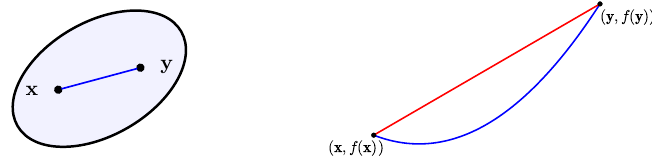
\includegraphics[width=0.8\textwidth]{images/convset.png}
 \caption{A convex set and a convex function}\label{fig:convfun}
\end{figure}

Convex function have pleasant properties, while at the same time covering many of the functions that arise in applications. Perhaps the most important property is that local minima are global minima.

\begin{theorem}
 Let $f\colon \R^n\to \R$ be a convex function. Then any local minimizer of $f$ is a global minimizer.
\end{theorem}

\begin{proof}
 Let $\vct{x}^*$ be a local minimizer and assume that it is not a global minimizer. Then there exists a vector $\vct{y}\in \R^d$ such that $f(\vct{y})<f(\vct{x}^*)$. Since $f$ is convex, for any $\lambda\in [0,1]$ and $\vct{x}=\lambda \vct{y}+(1-\lambda)\vct{x}^*$ we have
 \begin{equation*}
  f(\vct{x}) \leq \lambda f(\vct{y})+(1-\lambda) f(\vct{x}^*) < \lambda f(\vct{x}^*)+(1-\lambda)f(\vct{x}^*) = f(\vct{x}^*).
 \end{equation*}
This holds for all $\vct{x}$ on the line segment connecting $\vct{y}$ and $\vct{x}^*$. Since every open neighbourhood $U$ of $\vct{x}^*$ contains a bit of this line segment, this means that every open neighbourhood $U$ of $\vct{x}^*$ contains an $\vct{x}\neq \vct{x}^*$ such that $f(\vct{x})\leq f(\vct{x}^*)$, in contradiction to the assumption that $\vct{x}^*$ is a local minimizer. It follows that $\vct{x}^*$ has to be a global minimizer.
\end{proof}

\begin{remark} Note that in the above theorem we made no assumptions about the differentiability of the function $f$! In fact, while a convex function is always {\em continuous}, it need not be differentiable. The function $f(x) = |x|$ is a typical example: it is convex, but not differentiable at $x=0$.
\end{remark}

\begin{example}
 Affine functions $f(\vct{x})=\ip{\vct{x}}{\vct{a}}+b$ and the exponential function $e^x$ are examples of convex functions. 
\end{example}

\begin{example}
 In optimization we will often work with functions of matrices, where an $m\times n$ matrix is considered as a vector in $\R^{m\times n}\cong \R^{mn}$. If the matrix is symmetric, that is, if $\mtx{A}^{\trans}=\mtx{A}$, then we only care about the upper diagonal entries, and we consider the space $\mathcal{S}^n$ of symmetric matrices as a vector space of dimension $n(n+1)/2$ (the number of entries on and above the main diagonal). Important functions on symmetric matrices that are convex are the operator norm $\norm{\mtx{A}}_2$, defined as
 \begin{equation*}
  \norm{\mtx{A}}_2 := \max_{\vct{x}\colon \norm{\vct{x}}\leq 1} \frac{\norm{\mtx{A}\vct{x}}_2}{\norm{\vct{x}}_2},
 \end{equation*}
or the function $\log \det(\mtx{X})$, defined on the set of {\em positive semidefinite} symmetric matrices $\mathcal{S}_+^n$.
\end{example}

There are useful ways of characterising convexity using differentiability.
\begin{theorem}
\begin{enumerate}
 \item Let $f\in C^1(\R^n)$. Then $f$ is convex if and only if for all $\vct{x}, \vct{y}\in \R^n$,
 \begin{equation*}
  f(\vct{y})\geq f(\vct{x})+\nabla f(\vct{x})^{\trans} (\vct{y}-\vct{x}).
 \end{equation*}
 \item Let $f\in C^2(\R^n)$. Then $f$ is convex if and only if $\nabla^2 f(\vct{x})$ is positive semidefinite. If $\nabla^2f(\vct{x})$ is positive definite, then $f$ is strictly convex.
 \end{enumerate}
\end{theorem}

\begin{example}\label{ex:quad}
 Consider a quadratic function of the form
 
 \begin{equation*}
f(\vct{x}) = \frac{1}{2}\vct{x}^{\trans}\mtx{A}\vct{x}+\vct{b}^{\trans}\vct{x}+c, 
 \end{equation*}
 
 where $\mtx{A}\in \R^{n\times n}$ is symmetric. Writing out the product, we get
 
 \begin{align*}
   \mtx{x}^{T}\mtx{A}\vct{x} &= \begin{pmatrix} x_1 & \cdots & x_n
   \end{pmatrix}
   \begin{pmatrix}
   a_{11} & \cdots & a_{1n}\\
   \vdots & \ddots & \vdots\\
   a_{n1} & \cdots & a_{nn}
   \end{pmatrix}
   \begin{pmatrix}
   x_1\\ \vdots \\ x_n
   \end{pmatrix} \\
   &= \begin{pmatrix}
   x_1 & \cdots & x_n
   \end{pmatrix}
   \begin{pmatrix}
   a_{11}x_1+\cdots+a_{1n}x_n\\
   \vdots \\
   a_{n1}x_1+\cdots+a_{nn}x_n
   \end{pmatrix} = \sum_{i=1}^n \sum_{j=1}^n a_{ij} x_i x_j.
 \end{align*} 
 
 Because $\mtx{A}$ is symmetric, we have $a_{ij}=a_{ji}$, and the above product simplifies to
 
 \begin{equation*}
 \vct{x}^{T}\mtx{A}\vct{x} = \sum_{i=1}^n a_{ii} x_i^2 + 2\sum_{1\leq i<j\leq n} a_{ij}x_i x_j.
 \end{equation*}
 
 This is a quadratic function, because it involves products of the $x_i$. The gradient and the Hessian of $f(\vct{x})$ are found by computing the partial derivatives of $f$:
 
 \begin{equation*}
 \frac{\partial f}{\partial x_i} = \sum_{j=1}^n a_{ij} x_j + b_i, \quad \frac{\partial^2 f}{\partial x_i \partial x_j} = a_{ij}.
 \end{equation*}
 
 In summary, we have
 \begin{equation*}
   \nabla f(\vct{x}) = \mtx{A}\vct{x} + \vct{b}, \quad \nabla^2f(\vct{x}) = \mtx{A}.
 \end{equation*}
 
 Using the previous theorem, we see that $f$ is convex \textbf{if and only if} $\mtx{A}$ is positive semidefinite. A typical example for such a function is
 
 \begin{equation*}
   f(\vct{x}) = \|\mtx{A}\vct{x}-\vct{b}\|^2 = (\mtx{A}\vct{x}-\vct{b})^{T}(\mtx{A}\vct{x}-\vct{b}) = \vct{x}^{T}\mtx{A}^{T}\mtx{A}\vct{x} -2\vct{b}^{T}\mtx{A}\vct{x}+\vct{b}^T\vct{b}.
 \end{equation*}
 
 The matrix $\mtx{A}^T\mtx{A}$ is always symmetric and positive semidefinite (why?) so that the function $f$ is convex.
\end{example}

A convenient way to visualise a function $f\colon \R^2\to \R$ is through \textbf{contour plots}. A \textbf{level set} of the function $f$ is a set of the form
\begin{equation*}
  \{\vct{x}\mid f(\vct{x}) = c\},
\end{equation*}

where $c$ is the \textbf{level}. Each such level set is a curve in $\R^2$, and a contour plot is a plot of a collection of such curves for various $c$. If one colours the areas between adjacent curves, one gets a plot as in the following figure. A {\em convex function} is has the property that there is only one {\em sink} in the contour plot.

\begin{ipythonnb}
\\# import numpy as np
import numpy.linalg as la
import matplotlib.pyplot as plt
% matplotlib inline

# Create random data: we use the randn function
X = np.random.randn(3,2)
y = np.random.randn(3)

# Solve least squares problem minimize \|X\beta-y\|^2
# the index 0 says that we get the first component of the solution
# (the function lstsq give more output than just the beta vector)
beta = la.lstsq(X,y)[0]

# Create function and plot the contours
def f(a,b):
    return sum((a*X[:,0]+b*X[:,1]-y)**2)

# Find the "right" boundaries around the minimum
xx = np.linspace(beta[0]-8,beta[0]+8,100)
yy = np.linspace(beta[1]-8,beta[1]+8,100)
XX, YY = np.meshgrid(xx,yy)

Z = np.zeros(XX.shape)
for i in range(Z.shape[0]):
    for j in range(Z.shape[1]):
        Z[i,j] = f(XX[i,j],YY[i,j])

cmap = plt.cm.get_cmap("coolwarm")
plt.contourf(XX,YY,Z, cmap = cmap)
plt.show()
\end{ipythonnb}

\begin{figure}[h!]
\centering
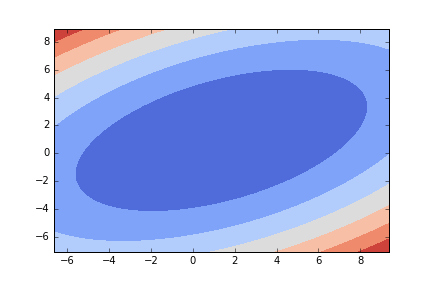
\includegraphics[width=0.6\textwidth]{images/contourplot.png}
\end{figure}


%-----------------------------------------------------------------------
% End of chap1.tex
%-----------------------------------------------------------------------


%\appendix
%\include{appendix1}

%\backmatter
%\include{biblio}
%\include{index}
\end{document}

%-----------------------------------------------------------------------
% End of chapter.tex
%-----------------------------------------------------------------------
